\chapter{Cài đặt công cụ cần thiết}
\label{Chapter1}

Để tiến hành biên dịch ứng dụng, ta cần cài đặt một số công cụ biên dịch và môi trường cần thiết.
\section{Cài đặt Apache Maven}
Apache Maven được dùng để biên dịch các service chạy Java Spring Boot: authentication; type-service; record-service; record-service; notification-service; service-registry; api-gateway.
    \subsection{Tải Java Development Kit (JDK)}
        Truy cập đường dẫn: \\
        \texttt{https://www.oracle.com/java/technologies/downloads/\#java17} \\
        
        để tiến hành tải về JDK cho tuỳ thuộc vào hệ điều hầnh (khuyến nghị phiên bản \textit{17+}).
    \subsection{Tải Apache Maven}
        Truy cập đường dẫn: \texttt{https://maven.apache.org/download.cgi}.
        Tại mục Files (Xem Hình ~\ref{fig:maven_download}), tiến hành tải xuống tệp có tên 
        
        \texttt{apache-maven-x.x.x-bin.zip} 
        
        (\texttt{x.x.x} là phiên bản Maven phù hợp, được khuyến nghị là \textit{3.9.6}).

        \begin{figure}
            \begin{center}
                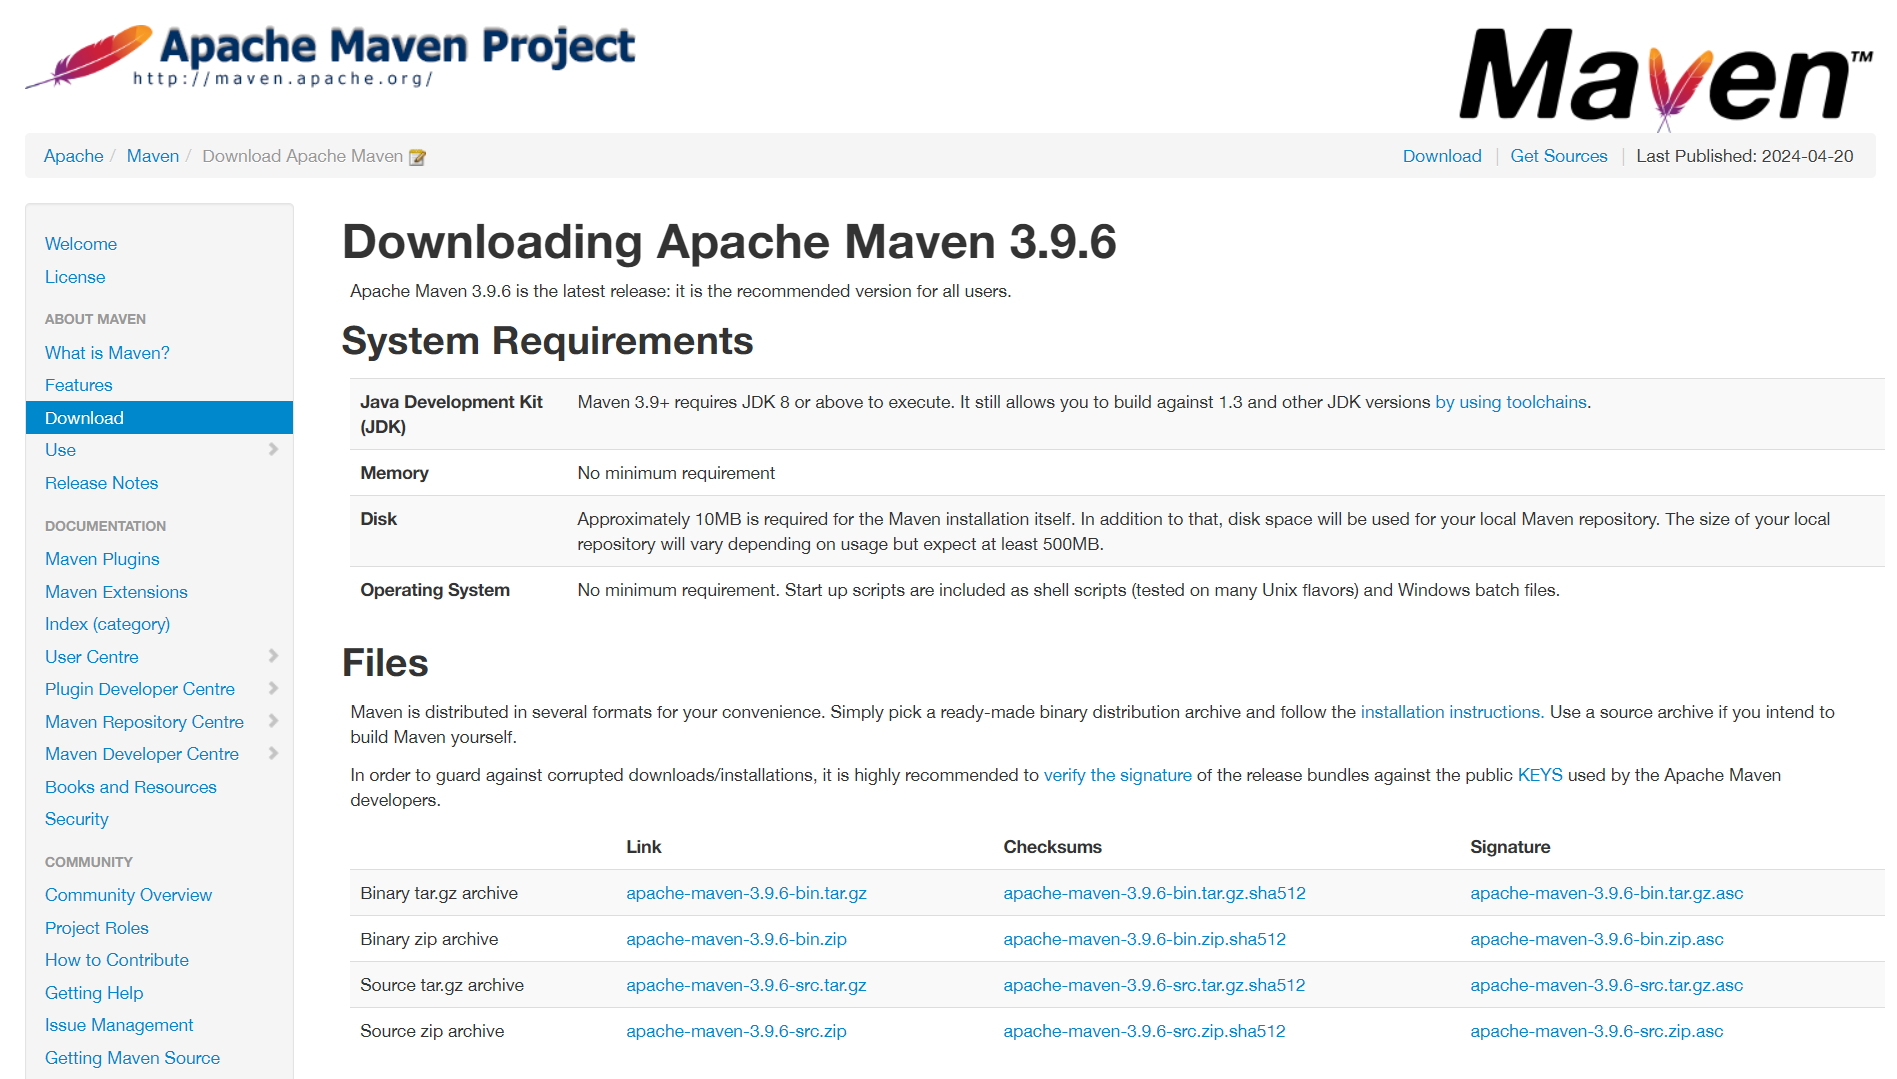
\includegraphics[width=1\linewidth]{maven_download.png}
                \caption{Màn hình tải về Apache Maven}
                \label{fig:maven_download}
            \end{center}
        \end{figure} 
    \subsection{Thêm biến môi trường}
        Sau khi đã tải về phiên bản Apache Maven như ý và giải nén. Thêm đường dẫn của thư mục \texttt{bin} vào biến môi trường.
    \subsection{Kết quả}
        Apache Maven được cài đặt thành công nếu như câu lệnh \texttt{mvn --version} chạy thành công.
    
\section{Cài đặt Node.js}
Node.js và Node Package Manager được sử dụng để cài đặt tất cả các dependencies, framework và library cần thiết cho việc biên dịch sản phẩm phía Frontend.

\subsection{Tải và cài đặt Node.js}
Truy cập đường link \texttt{https://nodejs.org/en/download}. Tải về và chạy file cài đặt Node.js tương ứng với hệ điều hành của mình.
(Xem Hình ~\ref{fig:node.js_download})

\begin{figure}
    \centering
    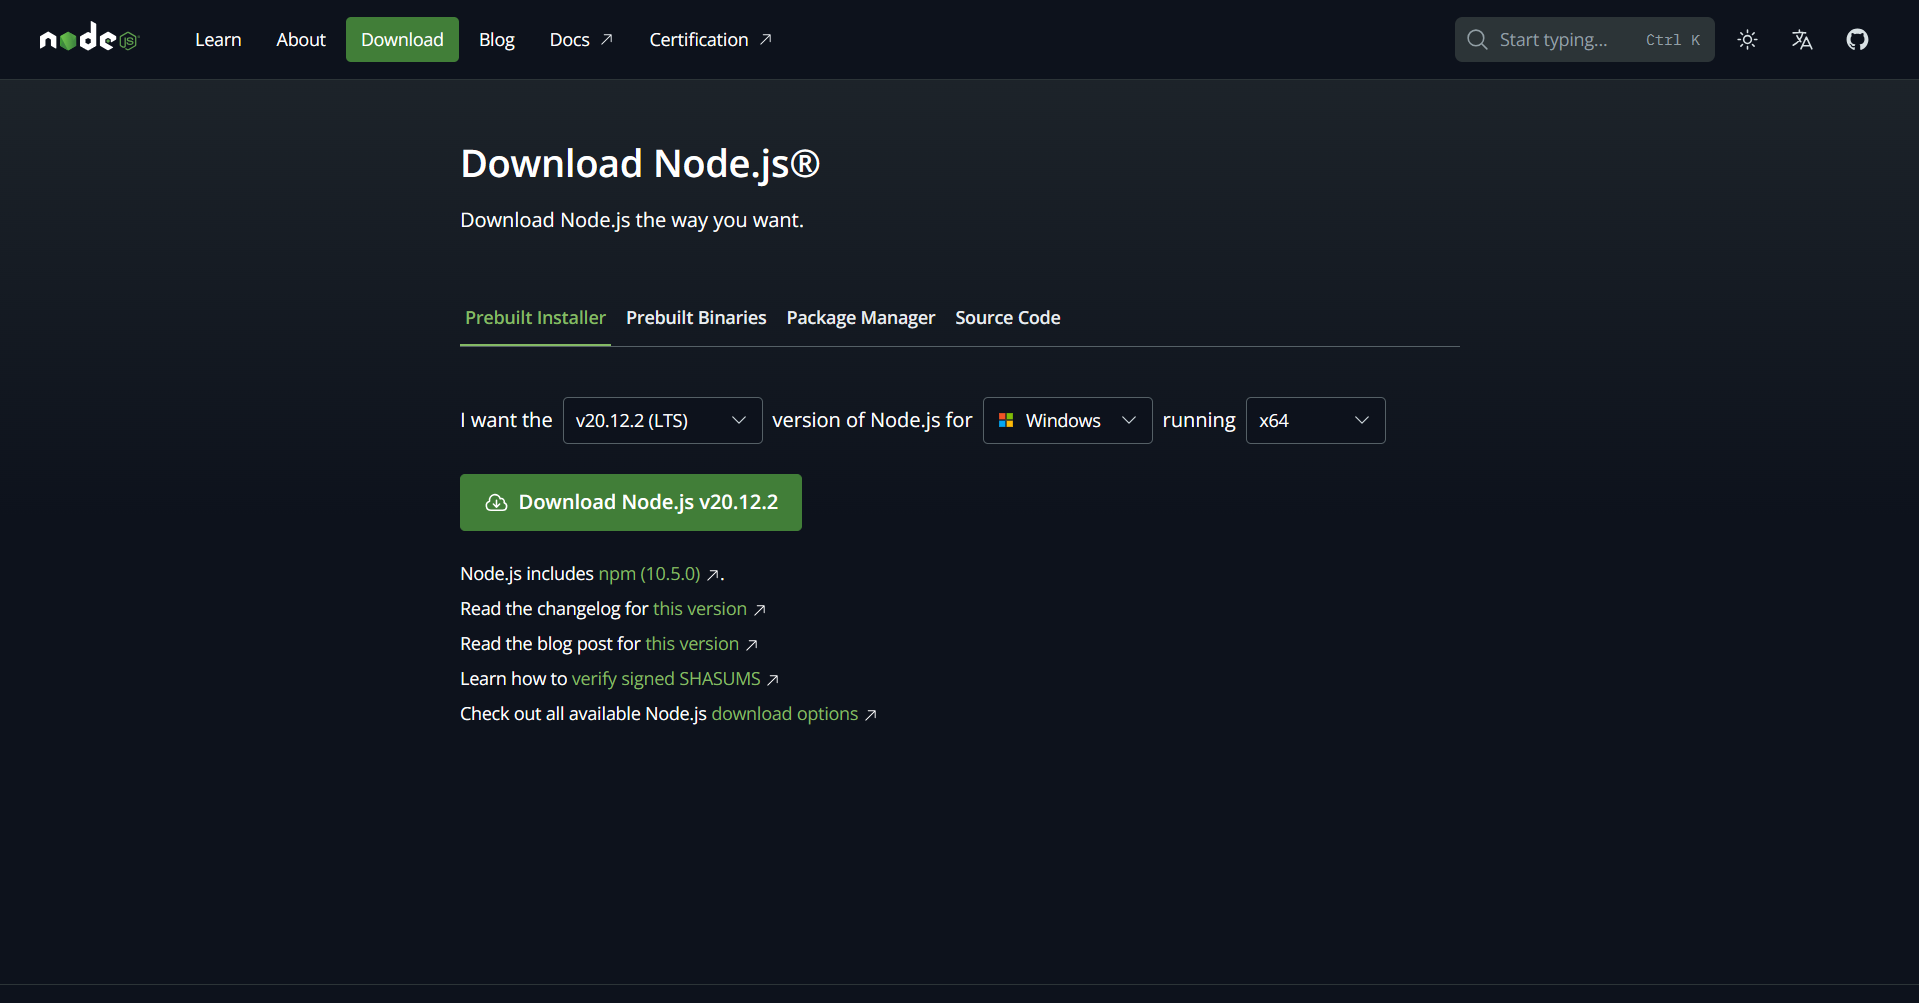
\includegraphics[width=1\linewidth]{nodejs_download.png}
    \caption{Màn hình tải về Node.js}
    \label{fig:node.js_download}
\end{figure}

\subsection{Kết quả}
Tương tự, nếu đã cài đặt thành công Node.js. Câu lệnh \texttt{node --version} sẽ được chạy thành công.
